\begin{abstract}
	On the MSc course "\textit{Computer Modelling Laboratory}" at ELTE, I've worked on a project in nuclear physics, where I studied the behaviour of the Japanese NEBULA detector and its response to neutron bombardment. For the simulation and analysis I've used the Geant4 general-purpose software, which is capable of producing state-of-the-art simulations and results in almost any field in nuclear- or particle physics.
\end{abstract}

\begin{multicols}{2}
\section{Introduction} \label{sec:1}
The NEBULA detector is a plastic scintillator array used to measure positions and momenta of neutrons between $100$ and $300$ MeV with high detection accuracy, large acceptance and sufficient position and velocity resolution\footnote{\url{http://be.nucl.ap.titech.ac.jp/~nebula/}}. To get a better grasp about the events inside a detector during an experiment - without actually running a neutron experiment - we're creating a computer simulation of the NEBULA detector with a more simplified structure in this project. To achieve this, I'm using the Geant4 simulation tool, developed for the simulation of the passage of particles through matter. In this environment I've implemented the NEBULA detector and a neutron beam to shoot at the detector. This report provides information about the status of this project at midterm.

\section{The Geant4 simulation tool} \label{sec:2}
The whole development of the project is done in the environment provided by the Geant4 software, developed by the Geant4 Collaboration at CERN. Its immense complexity, the comprehensive list of tools it offers and the way it operates, makes Geant4 an actual software developing job to use even at the most basic level. Besides the physical simulation capabilities it also offers an OpenGL+Qt backend for visualization, as well as a multi-threading support for both simulation and visualization purposes.

In this simulation engine environment one has the create a so called \texttt{World} geometry, in which all the events of the simulation happens. Anything leaving this volume during any part of the simulation, is rendered as non-existent for the time being. Inside the \texttt{World} box we can define other, smaller volumes in arbitrary shapes and sizes, which we can later fill with any predefined, or user-defined material at ease. These volumes will serve as the actual physical objects (targets, detectors, etc.) in a nuclear- or particle physics simulation. In this case I've implemented the NEBULA detector, along with an auxiliary neutron counter module for the early simulations.

The so called \texttt{particleGun} class was also used to create an arbitrary particle beam, shooting neutrons at the create NEBULA detector. In the following section I'm discussing the geometry and the particle beam in detail.
\begin{Figure}
	\centering
	\captionsetup{justification=centering}
	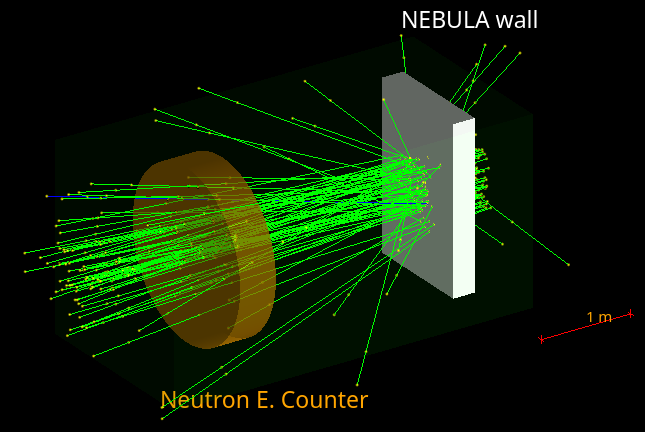
\includegraphics[width=\linewidth]{{images/nebula_3d.png}}
	\captionof{figure}{Geant4 simulation of the transit of 100 neutrons through a section of the NEBULA detector. The wall section of the NEBULA is colored white, while the bluish colored block is an auxiliary neutron energy counter (this latter is not present in case of the real NEBULA detector).} \label{fig:1}
\end{Figure}

\section{Geometry of the NEBULA detector} \label{sec:3}
The NEBULA detector is part of the Japanese SAMURAI beam line system at the RIKEN RI Beam Factory. It consist of $144$ plastic scintillator rods in total, all filled with the BC-$408$ scintillator material, consisting of $52.45\%$ of $H$ and $47.55\%$ of $C$. The rods are distributed equally on the two sides of the beam line with $60$ \texttt{NEUT} rods for neutron detection and $12$ \texttt{VETO} rods to detect charged particles on each side. In the project I'm only focused on to implement a section of one of the two walls in NEBULA and only the \texttt{NEUT} rods.
\begin{Figure}
	\centering
	\captionsetup{justification=centering}
	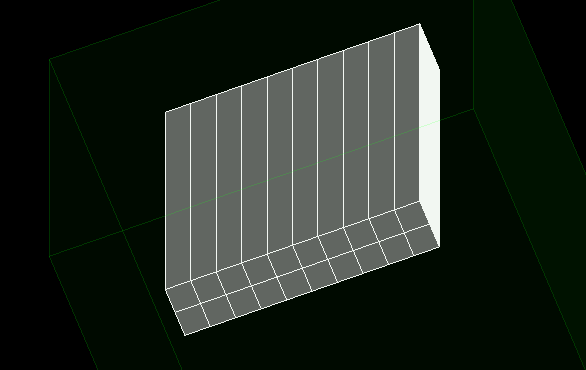
\includegraphics[width=\linewidth]{{images/nebula.png}}
	\captionof{figure}{The structure of the $20$ rods, $2$ layer section of the NEBULA detector viewed from above in the OpenGL+Qt visualization of the Geant4 simulation.} \label{fig:2}
\end{Figure}
On one side of the detector, there are $30-30$ \texttt{NEUT} scintillator rods organized in two layers. Neutrons hit the wall approximately perpendicular and deposits energy as they passes through the scintillator material. To simulate the process of neutron transit through this wall, it is enough to select a small section of it and simulate the bombardment of this part with perpendicular or near-perpendicular neutron beams. For this I've selected a $10$ rods wide (and $2$ rods deep) section of the wall, which I modelled using Geant4. The structure of this geometry can be seen in detail on Fig. \ref{fig:2}.

As seen on a Fig. \ref{fig:1}. and Fig. \ref{fig:3}., another volume called as \texttt{Neutron E. Counter} can be also seen. This structure is not present in case of the real NEBULA detector system, and now it is only there for debugging reasons.

\section{Particle beam} \label{sec:4}
The \texttt{particleGun} class from the Geant4 toolkit allows us to meticulously change every property of the inbound particles in the simulation. In the project I've only configured a neutron particle, and set the starting positions, momenta and energies of the spawned neutrons.

\subsection{Position} \label{ssec:4.1}
Starting positions of the simulated neutrons were sampled from the uniform distribution. Neutrons spawned inside a rectangular area not so far behind the detector wall (marked as \texttt{NEBULA wall} on Fig. \ref{fig:1}). The rectangle were approximately quarter of the size of the \texttt{NEBULA wall}. The $X$ and $Y$ coordinates (width and height respectively) were randomized, while the $Z$ coordinates (depth) was always at a fix location.

\subsection{Momentum} \label{ssec:4.2}
Similarly to positions, momentum values are also sampled from the uniform distribution. The biggest component in the momenta of particles, points into the direction of the negative $Z$ coordinate axis and guides the particles towards the neighbouring \texttt{NEBULA wall} block. A small inclination is randomly added to each of the particles, which is calculated by generating a uniformly random, small $X$ and $Y$ component for their momentum vector.

\subsection{Energy} \label{ssec:4.3}
The energy range of NEBULA is $100$ - $300$ MeV as in was mentioned in Sec. \ref{sec:1}. To prevent too much particle passing through the detector without any direction change, or negligible energy deposit,
while still staying in the real energy range, energies of all particles are uniformly set to $100$ MeV in the simulation.
\begin{Figure}
	\centering
	\captionsetup{justification=centering}
	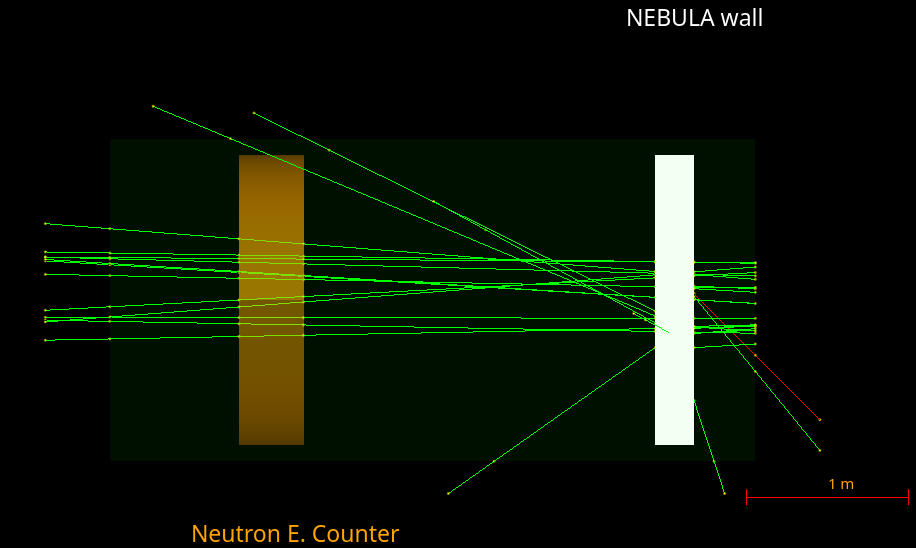
\includegraphics[width=\linewidth]{{images/nebula_2d.png}}
	\captionof{figure}{Geant4 simulation of the transit of $20$ neutrons through a section of the NEBULA detector. Same as Fig. \ref{fig:1}., but with only $20$ neutron and from side-view. Neutrons are spawned on the right side of the } \label{fig:3}
\end{Figure}

\section{Conclusions} \label{sec:5}
The reference for this project was the BSc thesis work of Dávid Pesznyák, who's discussed about the simplified implementation and analysis of various particle detectors using Geant4\footnote{\url{http://atomfizika.elte.hu/akos/tezisek/szd/pesznyakdavid_BScszd.pdf}}. In his thesis, the NEBULA detector and its response to neutron beams was also discussed. In the current state of the project, we can compare the image and behaviour of the shot target NEBULA wall, how particles scatters on and transits through it. Fig. 20. of the thesis is projects a clearly similar to those seen in this report on Fig. \ref{fig:1}. or on Fig. \ref{fig:3}.

This implies that the simulation I've created is working just as expected and ready for further expansions and analysis. The next step of the project will be to replicate other figures from mentioned thesis, like the energy deposit of neutrons in the rods of the NEBULA detector itself too.

\end{multicols}